\documentclass[11pt]{article}
\usepackage[utf8]{inputenc}
\usepackage{amssymb}
\usepackage{amsmath}
\usepackage{mathtools}
\usepackage{natbib}
\usepackage{xcolor}
\usepackage{listings}

\definecolor{cite}{rgb}{0.82, 0.1, 0.26}


\title{Aspect Based Sentiment Analysis}
\author{Saif Haq, acd17sh}
\date{November 2019}



\usepackage{natbib}
\usepackage{graphicx}

\begin{document}
\maketitle 
Supervisor: Prof. R.J. Gaizauskas\newline
Module Code: COM3610\newline
This report is submitted in partial fulfilment of the requirement for the degree of Computer Science by Saif Haq.\newline\newline


"All sentences or passages quoted in this report from other people's work have been specifically acknowledged by clear cross-referencing to author, work and page(s). Any illustrations that are not the work of the author of this report have been used with the explicit permission of the originator and are specifically acknowledged. I understand that failure to do this amounts to plagiarism and will be considered grounds for failure in this project and the degree examination as a whole."

-- Saif Haq, November 2019

\newpage
\tableofcontents
\newpage
\section{Introduction}
\section{Literature Survey}
\subsection{Aspect-Based Sentiment Analysis}
\textcolor{cite}{\citet{liu}} published a paper studying aspect-based sentiment analysis. The following definitions are fundamental to this field. 
\subsubsection{Definition: Entity} \label{def_entity}
An entity {$e$} is a product, service, person, event, organization, or topic. It is associated with a pair, $e$ : $(T,W)$, where $T$ is a hierarchy of components, sub-components, and so on, and $W$ is a set of attributes of $e$. Each component or sub-component also has its own set of attributes.

\subsubsection{Definition: Opinion} \label{def_opinion}
An opinion is a quintuple, $(e_i, a_{ij} , oo_{ijkl}, h_k, t_l)$
, where $e_i$ is the name of an entity, $a_{ij}$ is an aspect of $e_i$, $oo_{ijkl}$ is the sentiment on aspect $a_{ij}$, $h_k$ is the opinion holder, and $t_l$ is the time when the opinion is expressed by $h_k$. The sentiment $oo_{ijkl}$ can have positive, negative or neutral polarity with different strength levels. 

The goal of aspect-based sentiment analysis is to produce all opinion quintuples present in an opinionated document $D$.

\subsection{SemEval}
\textbf{Sem}antic \textbf{Eval}uation is an ongoing series of evaluations of computational semantic analysis systems, that aims to explore different natural language processing technologies through conferences, workshops and competitions. 
Task 5 of SemEval's annual workshop aims to tackle aspect based sentiment analysis, specially in the domain of customer reviews. They provide two datasets for this task for two domains of reviews: laptop reviews and restaurant reviews. This project will focus on their laptop laptop reviews datasets.  
% Aspect-based Sentiment analysis first appearing on SemEval's radar during their 2014 workshop, where the organisers provided datasets of reviews for ........... 
--More background will be added -- 

\subsection{Techniques for Aspect-Based Sentiment Analysis}
\subsubsection{Subjectivity Classification}
The goal of subjectivity classification is to distinguish whether a sentence $s$ expresses sentiment, or is objective. Sentiment and subjectivity are terms that can be used interchangeably.   
\subsubsection{Aspect Category Detection}
Aspect category detection is concerned with extracting aspects from a sentence $s$ which can be explicitly or implicitly defined. 1 explain techniques extracting aspect categories from user reviews.
\newline\newline
"This computer is really fast " $\rightarrow$  (computer)

Is an example of explicit aspect expression as computer is explicitly defined.
\newline\newline
"It is overpriced and the it dies quickly " $\rightarrow$ (price, battery life)

Is an example of an implicit aspect expression as the battery life is not explicitly defined. 
\newline\newline
 It can be difficult to define which category(s) a sentence falls under, especially due to incomplete domain coverage of categories. 
\newline\newline
% \textcolor{cite}{\citet{kim}} propose unsupervised and supervised techniques for achieving aspect category extraction. For their supervised method, probabilistic activation method, utilises an unsupervised method counting  
% \newline
\textcolor{cite}{\citet{tohsu}} implemented a deep learning technique via a single feed-forward neural network and a convolutional neural network using the input features as word embeddings. They also used Name List and Word
Cluster as input features but found these not to be particularly effective on testing data. This achieved the best results for Slot 1 of the SemEval 2016 Task 5 at the time of the competition. 
\newline\newline
However, \textcolor{cite}{\citet{acdgru}} have since achieved better results by employing a deep neural network based model utilising gated recurrent units as an encoder layer, a topic-attention layer, and a squash function which ouputs probabilities of each aspect category (\ref{gru}) for the SemEval 2014 and SemEval 2016 ASBA tasks . 

\subsubsection{Polarity Classification}
\textcolor{cite}{\citet{polaritywagner}} implemented a SVM with input feature word $n_{i=0}^{n=5}$ grams as well as features derived from scores assigned by a sentiment lexicon. They found that this significantly outperformed a lexical based approach, using token-distance; calculating the difference in the positions of the sentiment word and the aspect term by counting the tokens between them. 

\subsection{Approaches to Sentiment Analysis}
There are many different choices of techniques in addition to algorithms within these techniques for aspect based sentiment analysis (ASBA). Machine learning techniques can be supervised, semi-supervised, unsupervised and reinforcement. These techniques are described below \textcolor{cite}{\citet{hundred-page-machine-learning}}.

\paragraph{Supervised Learning}
In supervised learning, the dataset is the collection of labelled examples ${(x_i,y_i )_{i=1}^N}$. For each element $x_i$ among N is called a feature vector. If each example $x$ represents a person, the first feature $x^{(1)}$ could represent their weight in kg, the second feature $x^{(2)}$ could represent their height in cm, etc. The label $y_i$ can be an element belonging to a finite set of classes, Ie. for descriptions of a laptop, the classes could be ${(Battery Performance, Usability, ...)}$; or labels can be a more complex structure such as a vector, matrix or tree.  
The goal of a supervised learning algorithm is to use the dataset to produce a model that takes a feature vector $x$ as input and ouputs the information that allows deducing the label for this feature vector. 
\paragraph{Unsupervised Learning}
In unsupervised learning, the dataset is collection of unlabelled examples ${(x_i)_{i=1}^N}$ where $x$ is a feature vector. 
The goal of a supervised learning algorithm is to use the dataset to produce a model that takes a feature vector $x$ as input and ouputs a transformation of that feature vector that can be used to solve a problem. Clustering is an example that outputs the id of the cluster for each input ${x}$.
\paragraph{Semi-supervised Learning}
Semi-supervised learning contains both labelled and unlabelled examples, usually with a higher quantity of unlabelled examples. 
The goal of a semi-supervised learning algorithm is the same as supervised learning. 
\paragraph{Reinforcement Learning}
In reinforcement learning, the machine "lives" in an environment and perceives the state of the environment as feature vectors. Learning is done through trial and error, and a reward mechanism is employed with the goal being to learn a policy. A policy is a function that takes a feature vector as an input and ouputs an optimal action to execute that state. 
\newline\newline
This project will focus on supervised learning as this technique has seen a lot of success in the domain of aspect based sentiment analysis, and with the SemEval dataset to train and test on, multiple deep learning models will be created.

\newline\newline

\subsubsection{Support Vector Machines}
Support vector machines (SVMs) are a very powerful machine learning technique that aims to find an optimal hyper-plane in a multi-dimensional feature space that separates classes of data using a soft margin classifier, which determines the optimal distance between observations; and and a threshold \textcolor{cite}{\citet{cortesandvapnik1995}}. A soft margin classifier works when data isn't completely linearly separable, ie. allows misclassification through the use of slack variables (Observations on the wrong side of the optimal hyper-plane). A hard margin classifier on the other hand does not work when data isn't completely linearly separable \textcolor{cite}{\citet{boser}}. The name soft-margin comes from the fact that observations on the edge and within the soft margin are called support vectors. 
\newline\newline
Support vector machines use kernel functions to systematically find support vector classifiers in higher dimensions; which have the function of calculating the relationship between every pair of observation points as if they are in the higher dimensions, but they don't actually perform the transformations. This is known as the 'kernel trick, and is the reason why SVMs are fairly computationally cheap \textcolor{cite}{\citet{kernelfunctions}}. 
Two notable kernel functions are the polynomial function and radial based function. The polynomial kernel increases dimensions by setting a variable \textit{d}, the degree of the polynomial; whereas the radial based function finds support vector classifiers in infinite dimensions; behaving similar to a weighted nearest-neighbour classifier.
\newline\newline
\begin{figure}[h!]
\centering
\includegraphics[scale=1.2]{svm}
\caption{Support Vector machine optimal margin and optimal hyper-plane for a two-class classification problem in a 2-dimensional feature space}
\label{fig:svm}
\end{figure}
\newline

\subsubsection{Neural Networks}
The basic building block of a neural network is a neuron, commonly refereed to as a node. A node is a functional unit with input $U$ and output $Y$. Each node in a neural network can have different activation functions.
An activation function of a node defines the output $Y$ of that node given an input $U$. There are a vast variety of activation functions, each suited to different problems. Table \ref{tab:activation_functions} shows common activation functions.
Each connection between nodes has an arbitrary weight assigned to it. During training, these weights are constantly updated in attempts to reach their optimal value. 
\newline\newline
To train a neural network, a random sample of training inputs are chosen from the training data. A loss function is used to compute the errors for a prediction, and these are used by an optimisation algorithm to optimise weights. This is repeated until all training inputs are exhausted, which is said to complete an epoch of training. 
\newline 
The loss is the error between what the model is predicting for the training input, against the true label of the input. Stochastic gradient descent is a common optimisation algorithm. An optimisation algorithm has the aim of minimising a given loss function, by assigning the weights in a way to make this loss function as close to 0 as possible. It works by taking small steps in the direction of the steepest slope by calculating partial derivatives of the loss function; in an attempt to eventually reach the global minimum of said function. 
\textcolor{cite}{\citet{neuralnetworks}} 
\newline\newline
A widely used loss function is mean squared error, which calculates the square of difference between actual values and predicted values; however many different loss functions exist with their respected optimal domains. Cross entropy is a popular loss function for the domain of NLP. The modification of weights is said to use the backpropogation algorithm, as the error of the current node is propagated back to a previous layer.
\newline\newline
Adaptive Moment Estimation, or Adam is a recommended gradient descent optimization algorithm, however there are many others, with 9 of these algorithms being built into frameworks like TensorFlow.    
\newline\newline
\begin{table}[]
    \centering
    \begin{tabular}{ c|c }
        \hline
        \bf Activation function & 
        \bf Equation \\ \hline
        \\
        \bf Sigmoid & ${f(x) = \frac{1}{1+e^{-\beta x}}}$\\
        \\
        \hline
        \\
        \bf TanH & ${f(x) = \frac{2}{1+e^{-2x}}-1}$\\
        \\
        \hline
        \\
        \bf ReLU & 
        $   
        f(x) = 
             \begin{cases}
              \text{0,} &\quad\text{for x} \textless 0,\\
                \text{x,} &\quad\text{for x}  \ge0,\\
         
             \end{cases}
             
        $\\
        \\
        
        \hline
    \end{tabular}
    \caption{Common activation functions}
    \label{tab:activation_functions}
\end{table}

\paragraph{Artificial Neural Networks}
A deep neural network can be defined as a neural network with an input layer, an output layer and at least one hidden layer. Figure: \ref{fig:neuralnetwork}. This architecture of a neural network is a feed-forward network, where each neuron feeds data in one direction. Activations in one layer determine activations in the next layer. It is loosely analogous to how in biological networks of neurons, some groups of neurons firing cause other groups to fire. Neural networks are considered as universal function approximators meaning they can compute any function at all - activation functions allow non-linearity to exist within the network. \textcolor{cite}{\citet{wangann}} 
\newline\newline
\newline\newline
\begin{figure}[h!]
\centering
\includegraphics[scale=0.6]{neuralnetwork.png}
\caption{A feedforward artificial neural network.\newline Source: http://neuralnetworksanddeeplearning.com/chap1.html }
\label{fig:neuralnetwork}
\end{figure}
\newline


\subsubsection{Word Embeddings}
In NLP, the representation of words in a model still remains one of the predominant focuses of the field. \textcolor{cite}{\cite{mikolov}}'s word2vec library helped word embeddings become the predominant approach for vectorizing textual data, as it has proven that it significantly outperforms other methods of vectorization such as TF-IDF which indexes words on the basis of their frequencies in documents. Word embeddings work on the assumption that words with similar meanings appear in similar contexts, and capture this relation between words in their dense vector representation.
\newline
GloVe \textcolor{cite}{\cite{glove}} is a popular unsupervised learning algorithm packaged as a text file that provides vector representations of 400,000 words that were trained on a 2014 Wikipedia dump. The version referenced for this project contains embeddings in the dimensions: \{50, 100, 200, 300\}. \\

\paragraph{Convolutional Neural Networks}
Convolutional neural networks, (CNNs) are commonly used in image recognition tasks \textcolor{cite}{\citet{imagecnn}}. A CNN has convolutional layers which allow features to be extracted through a deep model of neurons. They are important where there is a translation invariance, ie. an entity in an image being able to be in different places. Despite being most known for image recognition, CNNs have proved powerful in other domains.  
Unlike an artificial neural network which takes vector inputs, CNNs take matrices as inputs. 
CNNs have filters which make them strong for pattern recognition. This could refer to edges in images near the beginning of the network, and possibly more sophisticated pattern recognition such as objects within the image; in the deeper of the convolutional layers.   
When a convolutional layer receives input, the filter will 'slide' over the set of inputs itself, known as convolving. After the filter has convolved the entire input, what is left is a new representation of the input, made up of dot products of the filters with input matrices. 
\newline\textbf{Pooling} is another operator that is typically added to CNNs following convolutional layers. There is max pooling, or average pooling that can be done. Both perform a dimensionality reduction from the convolved input's generated representation. Max pooling takes the max of the pixel values within the filter size, where average pooling takes the average. A stride determines how the filter moves across the pixels until an edge is reached, then the same is repeated one stride distance below. Reducing feature vectors reduces some computational expense which can translate to noticeable time saving when training the model.     
\paragraph{Recurrent Neural Networks}
Recurrent neural networks, (RNN) allow feedback loops between neurons, which is particularly useful for sequence data particularly temporal data, or where memory is desirable such as NLP tasks. The control flow of a RNN can be seen by Figure \ref{fig:rnn} \newline\newline
\newline\newline
Long short-term memory networks (LSTMs) and Gated Recurrent Units (GNUs) are popular types of RNNs that have been extensively used in the audio domain; making use of feedback loops to store memory within the network.

During back propagation, RNNs suffer from the vanishing gradient problem. This is when the gradient shrinks as it back propagates through time due to RNN's short-term memory; as a result of gradient variables becoming small to the point where their contribution to learning is negligible. 
\newline
Both LSTMs and GRUs have internal gates that regulate the flow of information combating RNNs traditional short term memory. Both LSTMs and GRUs can learn to keep track of important information and discard non-relevant data. This is what makes them a perfect neural networks for NLP tasks such as aspect based sentiment analysis. \textcolor{cite}{\citet{lstm}}.

\begin{figure}[h!]
\centering
\includegraphics[scale=0.4]{rnn.png}
\caption{Information flow in a Recurrent Neural Network \newline Source: http://colah.github.io/posts/2015-08-Understanding-LSTMs/}
\label{fig:rnn}
\end{figure}

\paragraph{Long Short Term Memory Networks} \label{lstm}

An LSTM has the same control flow as a recurrent neural network that passes data sequentially.
\textcolor{cite}{\citet{newcnns}} states that LSTMs contains a cell state that acts as a transport highway for relative information down the sequence chain. This is can be considered the "memory" of the network. As more inputs are passed into the LSTM, information gets added or removed to the cell state via gates. This can be seen on Figure \ref{fig:lstm}. Gates can learn what information to keep, and what information to discard during the training of the model. \newline\newline
As the cell state can carry information throughout the sequence process, information can in theory be carried from the first time step to the last time step. 

In a sequence of LSTM cells, a cell receives two inputs: a processed input vector (bottom), and a previous state vector (left). These two inputs are combined to make a single vector that is subsequently passed through a \textit{tanh} function that squashes values between -1 and +1; to regulate the output of the network.  

Gates within the LSTM contain \textit{sigmoid} activation functions, which squashes data between 0 and 1. Data that is not relevant to the problem domain will converge towards 0, and data that is important will converge towards 1. Inputs closer to 0 diminish after multiple back propagations. 


\begin{figure}[h!]
\centering
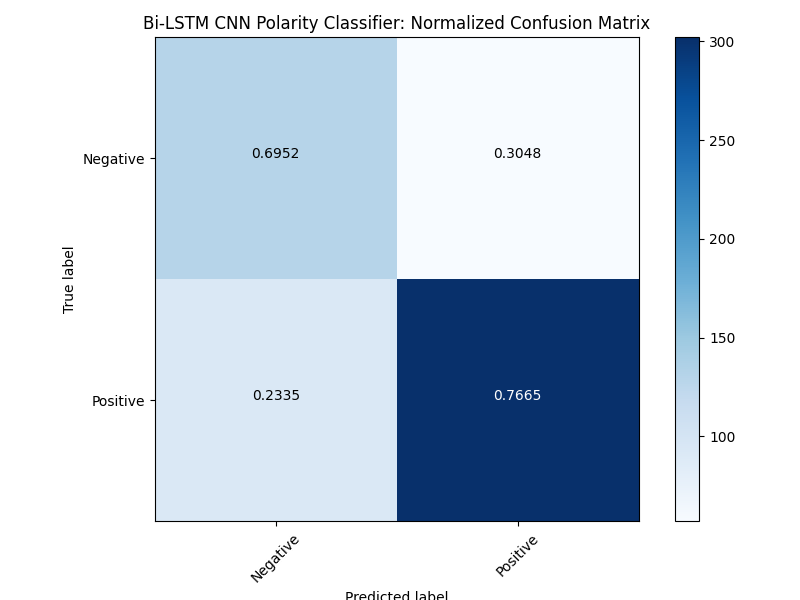
\includegraphics[scale=0.25]{lstm.png}
\caption{A LSTM cell and it's operations.\newline Source: https://towardsdatascience.com/illustrated-guide-to-lstms-and-gru-s-a-step-by-step-explanation-44e9eb85bf21}
\label{fig:lstm}
\end{figure}

\subsubsection{Hyperparameter Optimisation}
When implementing a deep learning model, hyperparameters will be encountered: such as the number of filters in a CNN, the amount of neurons in each hidden layer or even the number of layers the model has. \\
\paragraph{Grid search} is a 
\subsection{Libraries and Frameworks}
\subsubsection{Pandas}
Pandas is an open source library for Python that allows data manipulation and analysis. It is  well-suited to big data, and notably live data; hence its wide scale use in financial analysis applications.   
\subsubsection{Scikit-learn}
Scikit-learn is a popular open source library for Python that includes functions for various machine learning tasks, including data pre-processing and using feature vectors in machine learning algorithms such as support vector machines, random forests, K-nearest-neighbours etc. 
It also provides functions for model evaluation including metrics discussed in Section \ref{evaluationmeasures}.
  
\paragraph{Deep learning frameworks}

There is much debate online and within the research community as to what is the 'best' deep learning framework. The strengths and weaknesses of the three main competitors when writing this: Keras, TensorFlow, PyTorch are explained below. All three of the discussed deep learning frameworks are open-source. The frameworks operate on tensors and view any model as a directed acrylic graph, a finite directed graph with no directed circles; but differ on how you can define them.  
\subsubsection{TensorFlow}
TensorFlow is a high and low level deep learning API.

TensorFlow is by far the most popular deep learning framework, using GitHub activity as a metric. Google created it to help scale all of its' services including Google Translate, and now it has been adopted by some of the world's largest software companies including Airbnb, Snapchat, and Uber to mention a few. Having such a large community directly correlates to its' rich documentation and use in production environments; being commonly coupled with a Python web framework such as Django to serve machine learning to commercial users with ease. Using their tool: TensorFlow Serving, developers are easily able to serve their models at scale in production environments with distributed training. 
TensorBoard, is a visualisation tool for use with TensorFlow allowing developers to monitor the model training process. 
\newline
Developers define static computation graphs before compilation of the model; meaning all conditions and iterations in the graph structure have to be defined before it's run. Making changes in the neural networks structure means rebuilding it from scratch. Being built this way intentionally to maximise efficiency, does have the disadvantage of making debugging more difficult.

 
\subsubsection{PyTorch}
PyTorch is a low level deep learning framework, developed by Facebook to help power it's services, and is notably used by brands like Twitter and Salesforce. PyTorch using dynamic computation graphs as opposed to static, allows graphs to be created on the fly. It is commonly used for data analysis and is preferred for academic research as it is a low level framework. Debugging is fairly easy with PyTorch as a result of dynamic graphs, allowing developers to use common Python debugging techniques. It features declarative data parallelism, allowing it to achieve similar speeds to TensorFlow despite not using static computation graphs. It also comes with many pre-trained models; with some specifically trained for different NLP fields including sentiment analysis. Using Facebook's Caffee2 framework which is now merged into PyTorch, it is also production ready, although it isn't the favourite over TensorFlow for production environments.   

\subsubsection{Keras}
Keras is a minimalist library that can be run on top of TensorFlow, (or Microsoft's CNTK), which has support for a large range of neural network types and is favoured for its ease of use making it perfect for small scale projects or prototyping. It is great if the developer wishes not to understand as much about the computation that goes into making the model, and not needing to tune the model as much manually, or specifying the number of layers in the neural networks. For these reasons, it is not very well suited for research. 

Keras used to be used as a more high level approach to deep learning, however Google now have built Keras abstraction directly into TensorFlow.
This is now gives the benefit of levels of abstraction if needed for certain models, with the freedom to fine tune by accessing TensorFlows fine grained control of neural networks. 

It seems TensorFlow has a very bright future and clear lead in developing machine learning models; especially when going to production with TensorFlow Serving.

; but with TensorFlow2.0's release at the end of October 2019 this
\subsubsection{Chosen Deep Learning Framework}
I have chosen to opt for TensorFlow as the deep learning framework to implement neural networks for this project, mainly due to its wide-scale use in production environments. I believe TensorFlow will continue to grow and will remain the leading deep learning framework for years to come. 

\newpage
\section{Requirements and Analysis}

The focus of this project will be the cutting edge of ASBA, making use of different deep learning techniques. 

\subsection{Requirements}

% \begin{table}[]
%     \centering
%     \begin{tabular}{\textwidth}{{\extracolsep{\fill}}}
%         \bf Requirement & 
%         \bf Priority (10 High, 1, Low) \\ \hline
%         Implementation of a baseline for subjectivity classification & 9\\ \hline
%         Implementation of a baseline for aspect category detection & 8\\ \hline
%         Implementation of a baseline for opinion target extraction & 2\\ \hline
%         Implementation of a baseline for polarity classification & 5\\ \hline
%         Evaluation of baseline for subjectivity classification & 7\\ \hline
%         Evaluation of baseline for aspect category detection & 8\\ \hline
%         Evaluation of baseline for opinion target extraction & 7\\ \hline
%         Evaluation of baseline for polarity classification & 6\\ \hline  
        
%         Implementation of a deep-learning technique for subjectivity classification & 5\\ \hline
%         Implementation of a deep-learning technique for aspect category detection & 8\\ \hline
%         Implementation of a deep-learning technique for opinion target extraction & 8\\ \hline
%         Implementation of a deep-learning technique for polarity classification & 4\\ \hline
        
%         Evaluation of final system for subjectivity classification & 8\\ \hline
%         Evaluation of final system for aspect category detection & 8\\ \hline
%         Evaluation of final system for opinion target extraction & 8\\ \hline
%         Evaluation of final system for polarity classification & 6\\ \hline  
  
%         Experimentation with final system for subjectivity classification & 3\\ \hline
%         Experimentation with final system for aspect category detection & 7\\ \hline
%         Experimentation with final system for opinion target extraction & 7\\ \hline
%         Experimentation with final system for polarity classification & 2\\ \hline  

%         \hline
%     \end{tabular}
%     \caption{Requirements}
%     \label{tab:activation_functions}
% \end{table}

\subsection{Data Analysis}
\subsubsection{}
\begin{tabular}{llll}
\toprule
{} &               Opinions & Count & Percentage \\
\midrule
0 &            No Opinions &   461 &     18.44\% \\
1 &            One Opinion &  1352 &     54.08\% \\
2 &           Two Opinions &   534 &     21.36\% \\
3 &         Three Opinions &   127 &      5.08\% \\
4 &  Four or more opinions &    26 &      1.04\% \\
\bottomrule
\end{tabular}
\subsection{Evaluation Measures} \label{evaluationmeasures}
\subsection{Ethics}


\newpage

\section{Design}
\subsection{General System Architecture}
The laptops dataset that will be used for this project is available from SemEval in an XML format, so will need to be restructured so it can be utilised with Python. Each of the models implemented for this project will require their own pandas dataframe for training and testing data. For deep learning models, the training dataframe will have a random 20 percent taken to be the validation data. Preprocessed training data will be subject to feature extraction dependant on the task being tackled. The training phase will halt at an optimal epoch given by the loss calculated from the validation data. The validation data prevents overfitting of the network through early stopping. This is done through calculating the loss of the network for the training data and if it has not improved over $d$ epochs, the training will stop. \\
The final model will be serialized for used with future data, including the test data.  
\begin{figure}[t]
    \includegraphics[width=15cm]{arch.png}
    \caption{System architecture diagram}
    \centering
\end{figure}
\subsection{Standard Preprocessing}\label{preprocessing}
To improve accuracy of NLP models, textual data first needs to be preprocessed, with the goal being to leave only data that has a large impact on the classification of each sample. 
\begin{center}
    Text: \textit{Suffice it to say, my MacBook Pro keeps me going with its long battery life and blazing speed}.\\
\end{center}
The raw text above from the training dataset's sentence:292:2 first needs to be needs to be normalised, converting it all text to lower case. Next, the words need to be split from punctuation leaving the raw sentence text. Lastly, a stoplist is applied removing non-content words from the sentences. The example above will become:  

\begin{center}
    Text: \textit{suffice macbook pro long battery life blazing speed}
\end{center}

\subsection{Embedding Layer}
All of the deep learning models implemented for this project use Tensorflow's embedding layer to represent features in the input layer. For this layer to accept input data after standard preprocessing, the the text needs to be tokenized. A tokenizer object fits over training text and creates a dictionary of all words in the corpus, and maps them to an index. Sequences of input data are regarded as their index-dictionary mapping further down the input pipeline. Each word; now represented as a unique integer is replaced by an $d$ dimensional word embedding in the embedding layer. \\\\
Experiments will be conducted on the best use of different weights for the Embedding layer, being either random weights; fixed GloVe weights, or the use of GloVe weights as a seed, allowing the network to adjust the weights through back propagation. The impact of the dimensionality of word vector representations will also be explored.   

\subsection{Aspect Category Detection}
\subsubsection{Baseline SVM Model}
The first model developed for aspect category detection utilises a linear support vector classifier, as they have proven to perform effective in text classification tasks and make for a good baseline model. Sklearn's SGDClassifier is used in conjunction with the linear SVM, using the SVM to calculate a loss for each sample at a time; with the model being updated by performing stochastic gradient descent, maximising the performance of this linear classifier. \\

An effective sentiment analysis system needs to be able detect multiple opinions in single sentences, especially as 27.48\% of the training data was found to contain more than one opinion per sentence. To allow the baseline to achieve this, a model is created for each of the top 16 categories, with the output being the probability that a sample is in a given category or not; given by either a 1 or 0. Each of the sixteen models will perform separate classification on the data, and the results are joined at the end to analyse the performance of the models as a whole. 
The input of each model takes the standard preprocessed text described in \ref{preprocessing}, which feeds it into a sklearn pipeline object. In the pipeline, a CountVectorizer then a TfidfTransformer is applied. TFIDF has been a popular information retrieval method for many years, which combines term frequency with inverse document frequency, to reflect how import a word is to a document in the corpus, with the idea being that words that appear often in a document are less relevant to to its retrieval.   

\subsubsection{DNN Model}

The deep neural network model employs a global max pooling layer directly to the features from the embedding layer. This extracts the most salient features from every word embedding dimension, by taking the maximum value along each dimension of the word vectors \textcolor{cite}{\cite{baselinewordembeddings}}. This max pooling layer is fully connected to a 256-neuron dense layer with a ReLu activation function. The output layer has 16 neurons with sigmoid activations, calculating the probability a sample lies in each class.   

The labels are a one-hot encoded matrix, with each index corresponding to whether the sample lies in the index's category. Each label has a index assigned based on its frequency in the train dataset: so the \textit{LAPTOP\#GENERAL} label has an index of 0, (as it has 634 samples in the dataset); and \textit{KEYBOARD\#DESIGN\_FEATURES} has an index of 15 as it only has 29 samples in the train dataset. A sample containing exclusively these two labels is represented by the matrix: 
\begin{center}
    Labels:
    \textit{[1 0 0 0 0 0 0 0 0 0 0 0 0 0 0 1]}\\
\end{center}

\subsubsection{CNN Model}
\textcolor{cite}{\cite{yoonkim}} proposed a CNN be applied over multiple channels of feature vectors with different kernel sizes. The concatenation of the pooling of these layers showed to perform very well for various text categorization tasks. 
The CNN model developed for this project takes the feature vectors from the embedding layer and applies a Conv1D layer on each of the specified channels. Global max pooling is then applied to each of these channels before they are concatenated (See Figure \ref{embeddingconv}).
Each channel convolves over the input, extracting different n-gram features depending on the kernel size, which is different for each channel. Merged channels are then connected to an output layer of 16 neurons with a sigmoid activation function and dropout. Dropout is employed to act as further regularization in addition to early stopping \textcolor{cite}{\cite{dropout}}. Dropout layers are especially important when using a CNN, as convolutional layers increase the rate of convergence from feature vectors to labels for samples not in the training dataset. Channels further rate of increases overfitting, as each channel acts as an accelerator for feature convergence as the model is fed the same input multiple times over each channel; which is concatenated, so the model can be understood to train on each input sample multiple times per epoch. Dropout acts a blocker to certain neurons as activations attempt to pass through. This can be seen by seen by Figure \ref{dropout_img}. 

\begin{figure}[t]
    \begin{center}
        \includegraphics[width=14cm]{embeddingconv.png}
        \caption{CNN applied across multiple channels for feature vectors. \newline 
        Diagram adapted from \textcolor{cite}{\cite{yoonkim}}}
        \label{embeddingconv}
    \end{center}
\end{figure}

\begin{figure}[t]
    \begin{center}
    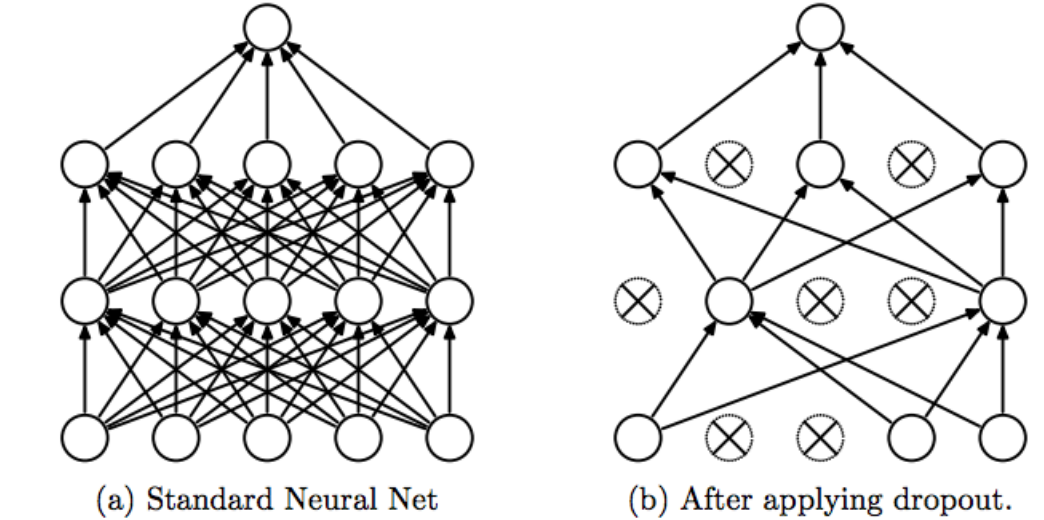
\includegraphics[width=12cm]{dropout.png}
    \caption{Dropout}
    \label{dropout_img}
    \end{center}
\end{figure}

\subsubsection{Bi-LSTM CNN Model}
\textcolor{cite}{\cite{clstm}} proposed an advancement of the prior CNN model by applying an LSTM to convolved feature vectors after concatenating the outputs from the different channel.s \\
The Bi-LSTM model implemented for this project takes inspiration from this project, but applies the Bidirectional LSTM directly to the feature vectors after the embedding layer. Multiple channels of different kernel sizes are applied to the concatenation of the LSTM output and the original embedding layer output. 
The rest of the model remains the same as the CNN model, with the convolved feature vectors being concatenated after max pooling, and then being connected to 16-neuron dense output layer with max pooling.  

To explore the best hyper-parameters of this model, a RandomSearch algorithm is employed to explore the search space. The library used for this is keras-tuner \cite{keras-tuner}. 
The search space to explore is the amount value 
The variable inputs are defined as 

\subsection{Subjectivity Classification}
\subsubsection{Baseline SVM Model}
\subsubsection{Bi-LSTM CNN Model}
The main model for subjectivity classification will use the same architecture proposed for aspect category detection, with the difference being the last layer of the network. 
\section{Implementation and Testing}

\subsection{Data Restructuring}
SemEval's datasets are provided in XML format, so need to be put into a pandas dataframe for interaction with python functions. The XML tree hierarchy can be seen from Figure \ref{fig:xml}. Each node in the tree has some attributes, with the sentence id, text, opinion aspect category(s) and affiliated polarity wanting to be transferred to the pandas dataframe.   

\begin{figure}[h!]
\begin{lstlisting}
<?xml version="1.0" encoding="UTF-8" standalone="yes"?>
<Reviews>
...
<Review rid="292">
    ...
    <sentence id="292:2">
        <text>Suffice it to say, my MacBook Pro keeps me going with 
            its long battery life and blazing speed.</text>
        <Opinions>
            <Opinion category="BATTERY#OPERATION_PERFORMANCE" 
                polarity="positive"/>
            <Opinion category="LAPTOP#OPERATION_PERFORMANCE" 
                polarity="positive"/>
        </Opinions>
    </sentence>
    ...
</Review>
...
</Reviews>
\end{lstlisting}
\label{fig:xml}
\caption{Example review from train dataset in XML format}
\end{figure}

To iterate through the XML tree, the \textit{xml.etree.ElementTree} module is used, with each sentence's text having standard preprocessing applied  (See Section \ref{preprocessing}). Depending on the task, a single sentence can be added multiple times with it's respective aspect/polarity tuple or subjectivity; or a single sentence can be added once, with relevant data regarding the task at hand. \\\\
Pandas allows for serialization of data in a .pkl file format. A pickle file is a binary serialization format that can store a variety of datatypes and has built in interaction with other modules such as numpy for dealing with matrices. It is also considerably faster than storing data as a CSV or JSON. 

\section{Results and Discussion}

\bibliographystyle{apa}
\bibliography{references}
\end{document}
